\chapter{未分类}

\begin{figure*}[htbp]
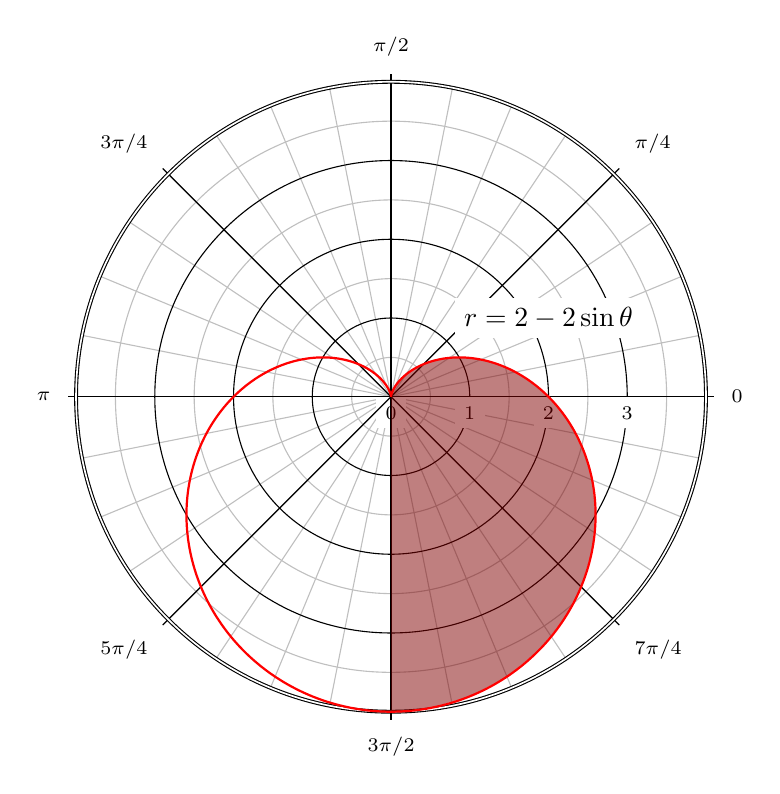
\begin{tikzpicture}[>=latex]

% Draw the lines at multiples of pi/12
\foreach \ang in {0,...,31} {
  \draw [lightgray] (0,0) -- (\ang * 180 / 16:4);
}

% Concentric circles and radius labels
\foreach \s in {0, 1, 2, 3} {
  \draw [lightgray] (0,0) circle (\s + 0.5);
  \draw (0,0) circle (\s);
  \node [fill=white] at (\s, 0) [below] {\scriptsize $\s$};
}

% Add the labels at multiples of pi/4
\foreach \ang/\lab/\dir in {
  0/0/right,
  1/{\pi/4}/{above right},
  2/{\pi/2}/above,
  3/{3\pi/4}/{above left},
  4/{\pi}/left,
  5/{5\pi/4}/{below left},
  7/{7\pi/4}/{below right},
  6/{3\pi/2}/below} {
  \draw (0,0) -- (\ang * 180 / 4:4.1);
  \node [fill=white] at (\ang * 180 / 4:4.2) [\dir] {\scriptsize $\lab$};
}

% The double-lined circle around the whole diagram
\draw [style=double] (0,0) circle (4);

\fill [fill=red!50!black, opacity=0.5] plot [domain=-pi/2:pi/2]
  (xy polar cs:angle=\x r, radius= {2-2*sin(\x r)});
\draw [thick, color=red, domain=0:2*pi, samples=200, smooth]
  plot (xy polar cs:angle=\x r, radius={2-2*sin(\x r)});
\node [fill=white] at (2,1) {$r=2-2\sin\theta$};

\end{tikzpicture} 
\end{figure*}

\begin{figure*}[htbp]
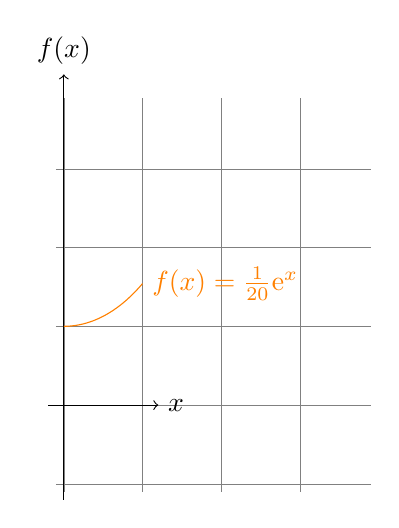
\begin{tikzpicture}[domain=0:1]
\draw[very thin,color=gray] (-0.1,-1.1) grid (3.9,3.9);
\draw[->] (-0.2,0) -- (1.2,0) node[right] {$x$};
\draw[->] (0,-1.2) -- (0,4.2) node[above] {$f(x)$};
% \x r means to convert ’\x’ from degrees to _r_adians:
% \draw[color=blue] plot (\x,{sin(\x r)}) node[right] {$f(x) = \sin x$};
\draw[color=orange] plot (\x,{0.5*(exp(\x) + exp(-\x))}) node[right] {$f(x) = \frac{1}{20} \mathrm e^x$};
\end{tikzpicture}

\end{figure*}

% -----------------------------------------------------------
\newpage

\begin{figure*}
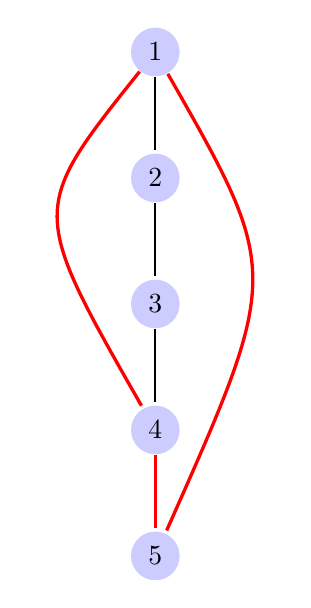
\begin{tikzpicture}[> = stealth, % arrow head style
	shorten > = 1pt, % don't touch arrow head to node
	auto,
	node distance = 3cm, % distance between nodes
	semithick % line style
	,scale=.8,auto=left,every node/.style={circle,fill=blue!20}]
	\node (n1) at (0,0)		{1};
	\node (n2) at (0,-2)  	{2};
	\node (n3) at (0,-4) 	{3};
	\node (n4) at (0,-6) 	{4};
	\node (n5) at (0,-8) 	{5};
	\draw (n1)--(n2);
	\draw (n2)--(n3);
	\draw (n3)--(n4);
	\draw [red,very thick](n4)--(n5);
	\draw [red,very thick] (n1) .. controls (-2,-2.5)  ..(n4);
	\draw [red,very thick](n1) .. controls (2,-3.5) 	..(n5);
	\end{tikzpicture}

\end{figure*}

% -----------------------------------------------------------
\newpage

\begin{figure*}
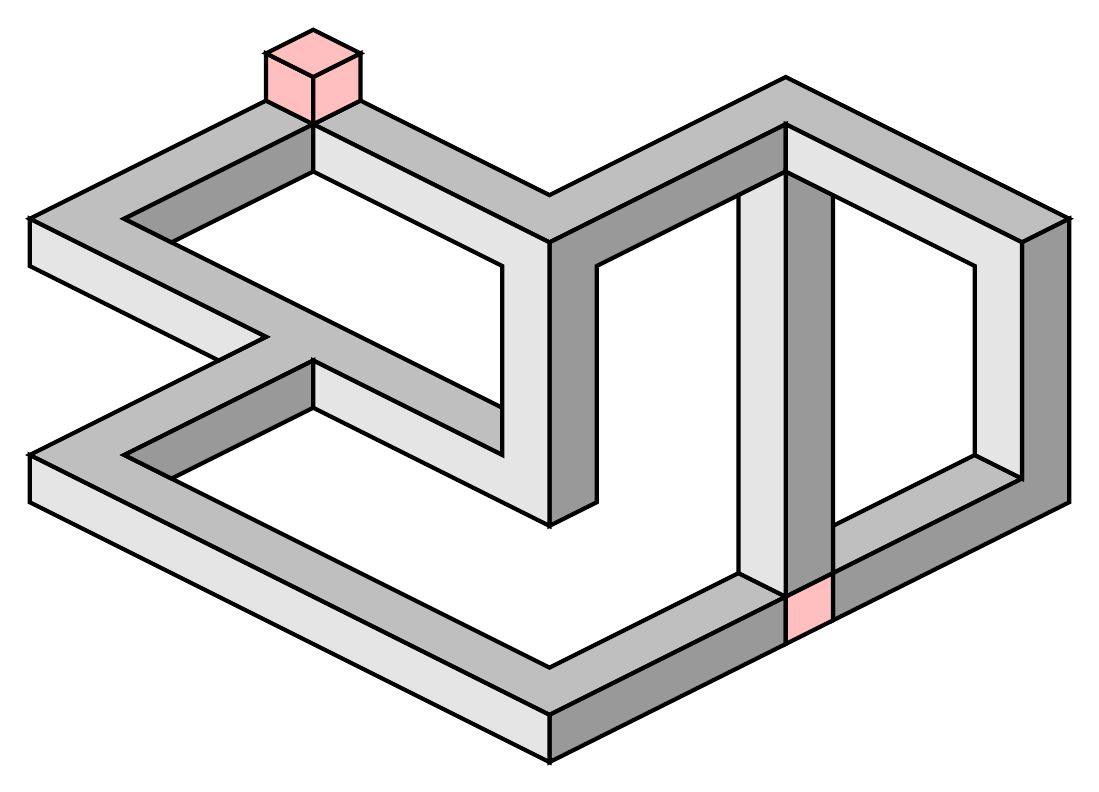
\begin{tikzpicture}[scale=1.5]
\definecolor{color1}{rgb}{0.9,0.9,0.9}
\definecolor{color3}{rgb}{0.75,0.75,0.75}
\definecolor{color2}{rgb}{0.6,0.6,0.6}
\coordinate[] (A1) at (-4.4,-0.2);
\coordinate[] (A2) at (-4.4,0.2);
\coordinate[] (A3) at (-4.4,1.8);
\coordinate[] (A4) at (-4.4,2.2);
\coordinate[] (B1) at (-4.0,2.0);
\coordinate[] (C1) at (-3.6,0.2);
\coordinate[] (C2) at (-3.6,2.2);
\coordinate[] (D1) at (-3.2,0);
\coordinate[] (D2) at (-3.2,2);
\coordinate[] (E1) at (-2.8,1);
\coordinate[] (F1) at (-2.4,1.2);
\coordinate[] (F2) at (-2.4,3.2);
\coordinate[] (F3) at (-2.4,3.6);
\coordinate[] (G1) at (-2,0.6);
\coordinate[] (G2) at (-2,1);
\coordinate[] (G3) at (-2,2.6);
\coordinate[] (G4) at (-2,3);
\coordinate[] (G5) at (-2,3.4);
\coordinate[] (G6) at (-2,3.8);
\coordinate[] (H1) at (-1.6,3.2);
\coordinate[] (H2) at (-1.6,3.6);
\coordinate[] (I1) at (-0.4,-0.2);
\coordinate[] (I2) at (-0.4,0.2);
\coordinate[] (I3) at (-0.4,0.6);
\coordinate[] (I4) at (-0.4,1.8);
\coordinate[] (J1) at (0,-2.4);
\coordinate[] (J2) at (0,-2);
\coordinate[] (J3) at (0,-1.6);
\coordinate[] (J4) at (0,-0.4);
\coordinate[] (J5) at (0,1.6);
\coordinate[] (J6) at (0,2);
\coordinate[] (J7) at (0,2.4);
\coordinate[] (K1) at (0.4,-0.2);
\coordinate[] (K2) at (0.4,1.8);
\coordinate[] (K3) at (0.4,2.2);
\coordinate[] (L1) at (1.6,-0.8);
\coordinate[] (L2) at (1.6,2.4);
\coordinate[] (M1) at (2,-1.4);
\coordinate[] (M2) at (2,-1);
\coordinate[] (M3) at (2,2.6);
\coordinate[] (M4) at (2,3);
\coordinate[] (M5) at (2,3.4);
\coordinate[] (N1) at (2.4,-1.2);
\coordinate[] (N2) at (2.4,-0.8);
\coordinate[] (N3) at (2.4,-0.4);
\coordinate[] (N4) at (2.4,2.4);
\coordinate[] (O1) at (3.6,0.2);
\coordinate[] (O2) at (3.6,1.8);
\coordinate[] (P1) at (4,0);
\coordinate[] (P2) at (4,2);
\coordinate[] (Q1) at (4.4,-0.2);
\coordinate[] (Q2) at (4.4,2.2);
\draw[line width=1.5pt,fill=color3] (A2)--(J2)--(M2)--(L1)--(J3)--(C1)--(G2)--(I2)--(I3)--(C2)--(G4)--(F2)--(A4)--(F1)--cycle;
\draw[line width=1.5pt,fill=color3] (N3)--(N2)--(P1)--(O1)--cycle;
\draw[line width=1.5pt,fill=color3] (Q2)--(M5)--(J7)--(H1)--(G4)--(J6)--(M4)--(P2)--cycle;
\draw[line width=1.5pt,fill=color2] (K1)--(J4)--(J6)--(M4)--(M3)--(K2)--cycle;
\draw[line width=1.5pt,fill=color2] (P2)--(P1)--(N2)--(N1)--(Q1)--(Q2)--cycle;
\draw[line width=1.5pt,fill=color2] (J2)--(J1)--(M1)--(M2)--cycle;
\draw[line width=1.5pt,fill=color2] (C2)--(D2)--(G3)--(G4)--cycle;
\draw[line width=1.5pt,fill=color2] (C1)--(D1)--(G1)--(G2)--cycle;
\draw[line width=1.5pt,fill=color2] (M3)--(M2)--(N2)--(N4)--cycle;
\draw[line width=1.5pt,fill=color1] (A4)--(A3)--(E1)--(F1)--cycle;
\draw[line width=1.5pt,fill=color1] (A2)--(A1)--(J1)--(J2)--cycle;
\draw[line width=1.5pt,fill=color1] (M3)--(M4)--(P2)--(P1)--(O1)--(O2)--cycle;
\draw[line width=1.5pt,fill=color1] (G4)--(G3)--(I4)--(I2)--(G2)--(G1)--(J4)--(J6)--cycle;
\draw[line width=1.5pt,fill=color1] (L2)--(L1)--(M2)--(M3)--cycle;
\draw[line width=1.5pt,fill=pink] (F3)--(F2)--(G4)--(G5)--cycle;
\draw[line width=1.5pt,fill=pink] (G5)--(G4)--(H1)--(H2)--cycle;
\draw[line width=1.5pt,fill=pink] (F3)--(G5)--(H2)--(G6)--cycle;
\draw[line width=1.5pt,fill=pink] (M1)--(N1)--(N2)--(M2)--cycle;

\end{tikzpicture}

\end{figure*}

% -----------------------------------------------------------
\newpage

xxx

\begin{figure*}[htbp]
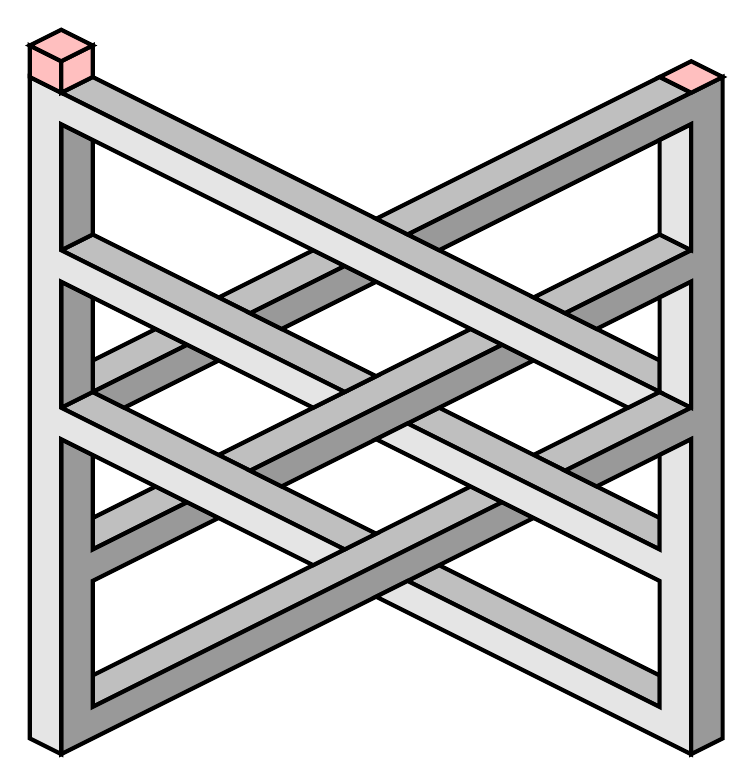
\begin{tikzpicture}[scale=1]
\definecolor{color1}{rgb}{0.9,0.9,0.9}
\definecolor{color3}{rgb}{0.75,0.75,0.75}
\definecolor{color2}{rgb}{0.6,0.6,0.6}
\coordinate[] (A1) at (-4.4,-4.2);
\coordinate[] (A2) at (-4.4,4.2);
\coordinate[] (A3) at (-4.4,4.6);
\coordinate[] (B1) at (-4,-4.4);
\coordinate[] (B2) at (-4,-0.4);
\coordinate[] (B3) at (-4,0);
\coordinate[] (B4) at (-4,1.6);
\coordinate[] (B5) at (-4,2);
\coordinate[] (B6) at (-4,3.6);
\coordinate[] (B7) at (-4,4);
\coordinate[] (B8) at (-4,4.4);
\coordinate[] (B9) at (-4,4.8);
\coordinate[] (C1) at (-3.6,-3.8);
\coordinate[] (C2) at (-3.6,-3.4);
\coordinate[] (C3) at (-3.6,-2.2);
\coordinate[] (C4) at (-3.6,-1.8);
\coordinate[] (C5) at (-3.6,-1.4);
\coordinate[] (C6) at (-3.6,-0.6);
\coordinate[] (C7) at (-3.6,0.2);
\coordinate[] (C8) at (-3.6,0.6);
\coordinate[] (C9) at (-3.6,1.4);
\coordinate[] (C10) at (-3.6,2.2);
\coordinate[] (C11) at (-3.6,3.4);
\coordinate[] (C12) at (-3.6,4.2);
\coordinate[] (C13) at (-3.6,4.6);
\coordinate[] (D1) at (-3.2,0);
\coordinate[] (E1) at (-2.8,-1);
\coordinate[] (E2) at (-2.8,1);
\coordinate[] (F1) at (-2.4,-1.2);
\coordinate[] (F2) at (-2.4,0.8);
\coordinate[] (G1) at (-2,-1.4);
\coordinate[] (G2) at (-2,-0.6);
\coordinate[] (G3) at (-2,0.6);
\coordinate[] (G4) at (-2,1.4);
\coordinate[] (H1) at (-1.6,-0.8);
\coordinate[] (H2) at (-1.6,1.2);
\coordinate[] (I1) at (-1.2,-1);
\coordinate[] (I2) at (-1.2,1);
\coordinate[] (J1) at (-0.8,-2);
\coordinate[] (J2) at (-0.8,0);
\coordinate[] (J3) at (-0.8,2);
\coordinate[] (K1) at (-0.4,-1.8);
\coordinate[] (K2) at (-0.4,0.2);
\coordinate[] (K3) at (-0.4,1.8);
\coordinate[] (L1) at (0,-2.4);
\coordinate[] (L2) at (0,-1.6);
\coordinate[] (L3) at (0,-0.4);
\coordinate[] (L4) at (0,0.4);
\coordinate[] (L5) at (0,1.6);
\coordinate[] (L6) at (0,2.4);
\coordinate[] (M1) at (0.4,-2.2);
\coordinate[] (M2) at (0.4,-0.2);
\coordinate[] (M3) at (0.4,2.2);
\coordinate[] (N1) at (0.8,-2);
\coordinate[] (N2) at (0.8,0);
\coordinate[] (N3) at (0.8,2);
\coordinate[] (O1) at (1.2,-1);
\coordinate[] (O2) at (1.2,1);
\coordinate[] (P1) at (1.6,-1.2);
\coordinate[] (P2) at (1.6,0.8);
\coordinate[] (Q1) at (2,-1.4);
\coordinate[] (Q2) at (2,-0.6);
\coordinate[] (Q3) at (2,0.6);
\coordinate[] (Q4) at (2,1.4);
\coordinate[] (R1) at (2.4,-0.8);
\coordinate[] (R2) at (2.4,1.2);
\coordinate[] (S1) at (2.8,-1);
\coordinate[] (S2) at (2.8,1);
\coordinate[] (T1) at (3.2,0);
\coordinate[] (U1) at (3.6,-3.8);
\coordinate[] (U2) at (3.6,-3.4);
\coordinate[] (U3) at (3.6,-2.2);
\coordinate[] (U4) at (3.6,-1.8);
\coordinate[] (U5) at (3.6,-1.4);
\coordinate[] (U6) at (3.6,-0.6);
\coordinate[] (U7) at (3.6,0.2);
\coordinate[] (U8) at (3.6,0.6);
\coordinate[] (U9) at (3.6,1.4);
\coordinate[] (U10) at (3.6,2.2);
\coordinate[] (U11) at (3.6,3.4);
\coordinate[] (U12) at (3.6,4.2);
\coordinate[] (V1) at (4,-4.4);
\coordinate[] (V2) at (4,-0.4);
\coordinate[] (V3) at (4,0);
\coordinate[] (V4) at (4,1.6);
\coordinate[] (V5) at (4,2);
\coordinate[] (V6) at (4,3.6);
\coordinate[] (V7) at (4,4);
\coordinate[] (V8) at (4,4.4);
\coordinate[] (W1) at (4.4,-4.2);
\coordinate[] (W2) at (4.4,4.2);
\draw[line width=1.5pt,fill=color3] (U7)--(U8)--(C12)--(B7)--cycle;
\draw[line width=1.5pt,fill=color3] (L6)--(M3)--(V7)--(U12)--cycle;
\draw[line width=1.5pt,fill=color3] (H2)--(K3)--(J3)--(G4)--cycle;
\draw[line width=1.5pt,fill=color3] (C7)--(F2)--(E2)--(C8)--cycle;
\draw[line width=1.5pt,fill=color3] (C5)--(C4)--(F1)--(E1)--cycle;
\draw[line width=1.5pt,fill=color3] (G2)--(H1)--(P2)--(O2)--cycle;
\draw[line width=1.5pt,fill=color3] (Q4)--(R2)--(V5)--(U10)--cycle;
\draw[line width=1.5pt,fill=color3] (R1)--(V3)--(U7)--(Q2)--cycle;
\draw[line width=1.5pt,fill=color3] (C2)--(C1)--(P1)--(O1)--cycle;
\draw[line width=1.5pt,fill=color3] (C10)--(B5)--(K2)--(L4)--cycle;
\draw[line width=1.5pt,fill=color3] (N2)--(M2)--(U4)--(U5)--cycle;
\draw[line width=1.5pt,fill=color3] (C7)--(B3)--(K1)--(L2)--cycle;
\draw[line width=1.5pt,fill=color3] (N1)--(M1)--(U1)--(U2)--cycle;
\draw[line width=1.5pt,fill=color2] (M3)--(N3)--(V6)--(V5)--(R2)--(S2)--(V4)--(V3)--(R1)--(S1)--(V2)--(V1)--(W1)--(W2)--cycle;
\draw[line width=1.5pt,fill=color2] (H2)--(I2)--(L5)--(K3)--cycle;
\draw[line width=1.5pt,fill=color2] (C7)--(D1)--(G3)--(F2)--cycle;
\draw[line width=1.5pt,fill=color2] (H1)--(I1)--(Q3)--(P2)--cycle;
\draw[line width=1.5pt,fill=color2] (B4)--(B3)--(C7)--(C9)--cycle;
\draw[line width=1.5pt,fill=color2] (B6)--(B5)--(C10)--(C11)--cycle;
\draw[line width=1.5pt,fill=color2] (B2)--(B1)--(Q1)--(P1)--(C1)--(C3)--(G1)--(F1)--(C4)--(C6)--cycle;
\draw[line width=1.5pt,fill=color1] (U11)--(U10)--(V5)--(V6)--cycle;
\draw[line width=1.5pt,fill=color1] (U9)--(U7)--(V3)--(V4)--cycle;
\draw[line width=1.5pt,fill=color1] (V2)--(U6)--(U4)--(M2)--(L3)--(U3)--(U1)--(M1)--(L1)--(V1)--cycle;
\draw[line width=1.5pt,fill=color1] (T1)--(U7)--(A2)--(A1)--(B1)--(B2)--(J1)--(K1)--(B3)--(B4)--(J2)--(K2)--(B5)--(B6)--cycle;
\draw[line width=1.5pt,fill=pink] (U12)--(V7)--(W2)--(V8)--cycle;
\draw[line width=1.5pt,fill=pink] (A3)--(A2)--(B7)--(B8)--cycle;
\draw[line width=1.5pt,fill=pink] (B8)--(B7)--(C12)--(C13)--cycle;
\draw[line width=1.5pt,fill=pink] (B9)--(A3)--(B8)--(C13)--cycle;
\end{tikzpicture}

\end{figure*}

YYY

% -----------------------------------------------------------
\newpage

A Cone in 3D

\begin{figure*}[htbp]
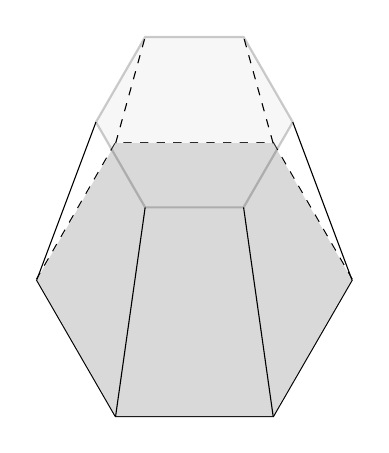
\begin{tikzpicture}[]
\def\RI{2}
\def\RII{1.25}

\draw[thick] (\RI,0)
  \foreach \x in {0,300,240,180} { --  (\x:\RI) node at (\x:\RI) (R1-\x) {} };
\draw[dashed,thick] (R1-0.center)
  \foreach \x in {60,120,180} { --  (\x:\RI) node at (\x:\RI) (R1-\x) {} };
\path[fill=gray!30] (\RI,0)
  \foreach \x in {0,60,120,180,240,300} { --  (\x:\RI)};

\begin{scope}[yshift=2cm]
\draw[thick,fill=gray!30,opacity=0.2] (\RII,0)
  \foreach \x in {0,60,120,180,240,300,360} { --  (\x:\RII) node at (\x:\RII) (R2-\x) {}};
\end{scope}

\foreach \x in {0,180,240,300} { \draw (R1-\x.center)--(R2-\x.center); };
\foreach \x in {60,120} { \draw[dashed] (R1-\x.center)--(R2-\x.center); };
\end{tikzpicture}
\end{figure*}


\begin{figure*}[htbp]
\tikzset{
	MyPersp/.style={scale=1.8,x={(-0.8cm,-0.4cm)},y={(0.8cm,-0.4cm)},
    z={(0cm,1cm)}},
%  MyPersp/.style={scale=1.5,x={(0cm,0cm)},y={(1cm,0cm)},
%    z={(0cm,1cm)}}, % uncomment the two lines to get a lateral view
	MyPoints/.style={fill=white,draw=black,thick}
		}
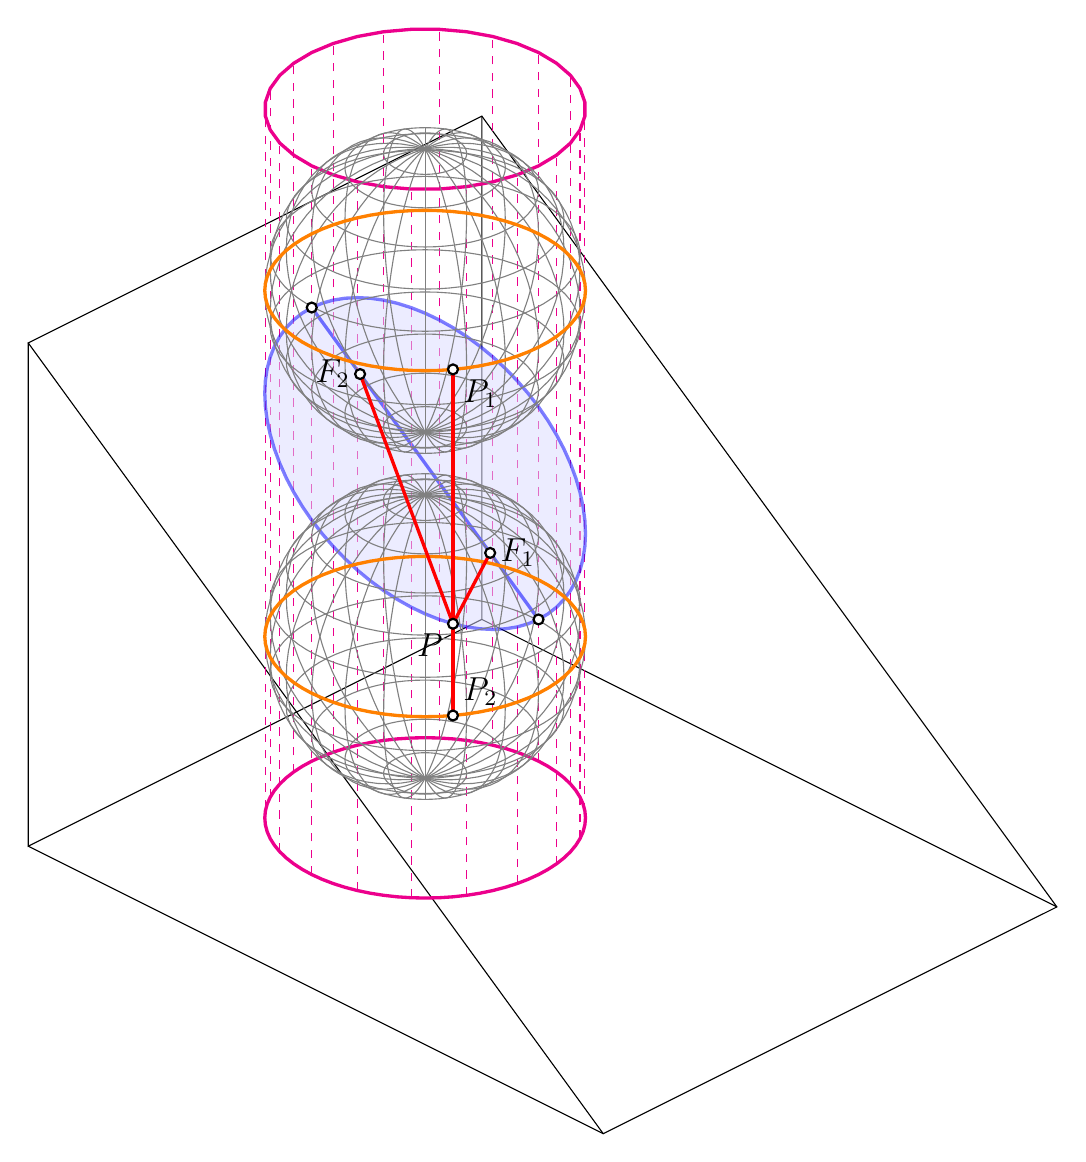
\begin{tikzpicture}[MyPersp,font=\large]
	% the base circle is the unit circle in plane Oxy
	\def\h{2.5}% Heigth of the ellipse center (on the axis of the cylinder)
	\def\a{35}% angle of the section plane with the horizontal
	\def\aa{35}% angle that defines position of generatrix PA--PB
	\pgfmathparse{\h/tan(\a)}
  \let\b\pgfmathresult
	\pgfmathparse{sqrt(1/cos(\a)/cos(\a)-1)}
  \let\c\pgfmathresult %Center Focus distance of the section ellipse.
	\pgfmathparse{\c/sin(\a)}
  \let\p\pgfmathresult % Position of Dandelin spheres centers
                       % on the Oz axis (\h +/- \p)
	\coordinate (A) at (2,\b,0);
	\coordinate (B) at (-2,\b,0);
	\coordinate (C) at (-2,-1.5,{(1.5+\b)*tan(\a)});
	\coordinate (D) at (2,-1.5,{(1.5+\b)*tan(\a)});
	\coordinate (E) at (2,-1.5,0);
	\coordinate (F) at (-2,-1.5,0);
	\coordinate (CLS) at (0,0,{\h-\p});
	\coordinate (CUS) at (0,0,{\h+\p});
	\coordinate (FA) at (0,{\c*cos(\a)},{-\c*sin(\a)+\h});% Focii
	\coordinate (FB) at (0,{-\c*cos(\a)},{\c*sin(\a)+\h});
	\coordinate (SA) at (0,1,{-tan(\a)+\h}); % Vertices of the
                                           % great axes of the ellipse
	\coordinate (SB) at (0,-1,{tan(\a)+\h});
	\coordinate (PA) at ({sin(\aa},{cos(\aa)},{\h+\p});
	\coordinate (PB) at ({sin(\aa},{cos(\aa)},{\h-\p});
	\coordinate (P) at ({sin(\aa)},{cos(\aa)},{-tan(\a)*cos(\aa)+\h});
     % Point on the ellipse on generatrix PA--PB

	\draw (A)--(B)--(C)--(D)--cycle;
	\draw (D)--(E)--(F)--(C);
	\draw (A)--(E) (B)--(F);
	\draw[blue,very thick] (SA)--(SB);

%	\coordinate (O) at (0,0,0);
%	\draw[->] (O)--(2.5,0,0)node[below left]{x};
%	\draw[->] (O)--(0,3,0)node[right]{y};
%	\draw[->] (O)--(0,0,6)node[left]{z};

	\foreach \t in {20,40,...,360}% generatrices
		\draw[magenta,dashed] ({cos(\t)},{sin(\t)},0)
      --({cos(\t)},{sin(\t)},{2.0*\h});
	\draw[magenta,very thick] (1,0,0) % lower circle
		\foreach \t in {5,10,...,360}
			{--({cos(\t)},{sin(\t)},0)}--cycle;
	\draw[magenta,very thick] (1,0,{2*\h}) % upper circle
		\foreach \t in {10,20,...,360}
			{--({cos(\t)},{sin(\t)},{2*\h})}--cycle;
	\fill[blue!15,draw=blue,very thick,opacity=0.5]
     (0,1,{\h-tan(\a)}) % elliptical section
		\foreach \t in {5,10,...,360}
			{--({sin(\t)},{cos(\t)},{-tan(\a)*cos(\t)+\h})}--cycle;

	\foreach \i in {-1,1}{%Spheres!
		\foreach \t in {0,15,...,165}% meridians
			{\draw[gray] ({cos(\t)},{sin(\t)},\h+\i*\p)
				\foreach \rho in {5,10,...,360}
					{--({cos(\t)*cos(\rho)},{sin(\t)*cos(\rho)},
          {sin(\rho)+\h+\i*\p})}--cycle;
			}
		\foreach \t in {-75,-60,...,75}% parallels
			{\draw[gray] ({cos(\t)},0,{sin(\t)+\h+\i*\p})
				\foreach \rho in {5,10,...,360}
					{--({cos(\t)*cos(\rho)},{cos(\t)*sin(\rho)},
          {sin(\t)+\h+\i*\p})}--cycle;
			}
					\draw[orange,very thick] (1,0,{\h+\i*\p})% Equators
		\foreach \t in {5,10,...,360}
			{--({cos(\t)},{sin(\t)},{\h+\i*\p})}--cycle;
		}
	\draw[red,very thick] (PA)--(PB);
	\draw[red,very thick] (FA)--(P)--(FB);
%	\fill[MyPoints] (CLS) circle (1pt);% center of lower sphere
%	\fill[MyPoints] (CUS) circle (1pt);% center of upper sphere
	\fill[MyPoints] (FA) circle (1pt)node[right]{$F_1$};
	\fill[MyPoints] (FB) circle (1pt)node[left]{$F_2$};
	\fill[MyPoints] (SA) circle (1pt);
	\fill[MyPoints] (SB) circle (1pt);
	\fill[MyPoints] (P) circle (1pt)node[below left]{$P$};
	\fill[MyPoints] (PA) circle (1pt)node[below right]{$P_1$};
	\fill[MyPoints] (PB) circle (1pt)node[above right]{$P_2$};
\end{tikzpicture}
\end{figure*}









